% % % % % % % % % % % % % % % % % % % % % % % % % % % % % % % % % % % % % % % % 
% Formelsammlung von LaTeX4EI									
%
% @encode: 	UTF-8, tabwidth = 4, newline = LF
% @author:	Lukas Kompatscher, Samuel Harder (orginal von Emanuel Regnath, Martin Zellner, Alexander Preißner und Hendrik Böttcher)
% @date:		
%
% % % % % % % % % % % % % % % % % % % % % % % % % % % % % % % % % % % % % % % % 

%---------------------------------------%
%		Stochastische Signale			%
%~~~~~~~~~~~~~~~~~~~~~~~~~~~~~~~~~~~~~~~%

% Document Class ===============================================================
\documentclass[german,color,6pt]{latex4ei/latex4ei_sheet}

% set document information
\title{Stochastische \\ Signale}
\author{Emanuel Regnath, Martin Zellner, Alexander Preißner, Hendrik Böttcher, Lukas Kompatscher, Samuel Harder}	
\myemail{samuel.harder@tum.de}	

\DeclareMathOperator{\W}{\textit{W}}				% Zufallsvariable W
\DeclareMathOperator{\U}{\textit{U}}				% Zufallsvariable U
\DeclareMathOperator{\V}{\textit{W}}				% Zufallsvariable V

\DeclareTextFontCommand{\emph}{\bfseries}

% Dokumentbeginn
% ======================================================================
\begin{document}
	
	\maketitle
	
	% SECTION ====================================================================================
	\section{Mengenalgebra}
	% ============================================================================================
	\begin{sectionbox}
		\subsection{Mengen- und Boolsche Algebra}
		\begin{tablebox}{lll}
			%& $(P(\Omega);\capdot , \cupplus, \overline{A};\Omega,\emptyset )$\\ \mrule
			Kommutativ 		& $A \capdot B = B \capdot A$ & $A \cupplus B = B \cupplus A$\\
			Assoziativ 		& \multicolumn{2}{l}{ $(A \capdot B) \capdot C = A \capdot (B \capdot C)$} \\
			& \multicolumn{2}{l}{$(A \cupplus B) \cupplus C = A \cupplus (B \cupplus C)$} \\
			Distributiv 	& \multicolumn{2}{l}{$A \capdot (B \cupplus C) = (A \capdot B) \cupplus (A \capdot C)$}\\
			& \multicolumn{2}{l}{ $A \cupplus (B \capdot C) = (A \cupplus B) \capdot (A \cupplus C)$}\\ \cmrule
			Indempotenz		& $A \capdot A = A$ & $A \cupplus A = A$\\
			Absorbtion		& $A \capdot (A \cupplus B) = A$ & $A \cupplus (A \capdot B) = A$\\
			Neutralität		& $A \capdot \Omega = A$ & $A \cupplus \emptyset = A$\\
			Dominant		& $A \capdot \emptyset = \emptyset$ & $A \cupplus \Omega = \Omega$\\
			Komplement		& $A \capdot \overline{A} = \emptyset$ & $A \cupplus \overline{A} = \Omega$\\
			& $\overline{\overline{A}} = A$ & $\ol{\Omega} = \emptyset$\\
			De Morgan		& $\overline{A \capdot B} = \overline{A} \cupplus \overline{B}$ & $\overline{A \cupplus B} = \overline{A} \capdot \overline{B}$\\
		\end{tablebox}
	\end{sectionbox}
	

\begin{sectionbox}
	\subsection{Kombinatorik}
	Mögliche Variationen/Kombinationen um $k$ Elemente von maximal $n$ Elementen zu wählen bzw. $k$ Elemente auf $n$ Felder zu verteilen:
	\begin{tablebox}{l|cc}
		& \large Mit Reihenfolge & \large Reihenfolge egal\\ \cmrule
		%& ungleiche Elemente & gleiche Elemente \\ 
		\large Mit Wiederholung & \large $n^k$ & \Large $\binom{n+k-1}{k}$\\[0.2em]
		\large Ohne Wiederholung & \Large $\frac{n!}{(n-k)!}$ & \Large $\binom nk$\\
	\end{tablebox}
	Permutation von $n$ mit jeweils $k$ gleichen Elementen: $\frac{n!}{k_1 ! \cdot k_2 ! \cdot ...}$ \\
	$\binom nk = \binom n{n-k} = \frac{n!}{k! \cdot (n-k)!}$ \quad $\binom 42 = 6$ \quad $\binom 52 = 10$
\end{sectionbox}

%Methode: Mengen so zerlegen, dass sie disjunkt sind, nur dann ist die Mengensumme(Vereinigung) auch die arithmeitsche Summe(+):
%$\P(A \cup B) = \P(A\setminus B)+\P(B) = \P(A) + \P(B) - \P(A \cap B)$\\
\begin{sectionbox}
	\subsection{Grundbegriffe}
	
	\begin{tablebox}{ll}
		Tupel & $(i,j) \neq (j,i)$ für $i \neq j$ \\
		Ungeordnetes Paar & $\{i,j\} = \{j,i\}$ \\
		Potenzmenge & $\mathbb \P(\Omega)$ ist Menge aller Teilmengen von $\Omega$ \\
	\end{tablebox}
\end{sectionbox}

\begin{sectionbox}
	\subsection{Integralarten}
	
	\renewcommand{\arraystretch}{1.6} 
	\begin{tablebox}{ccc}
		$F(x)$ & $f(x)$ & $f'(x)$ \\ \cmrule
		$\frac{1}{q+1}x^{q+1}$ & $x^q$ & $qx^{q-1}$ \\
		\raisebox{-0.2em}{$\frac{2\sqrt{ax^3}}{3}$} & $\sqrt{ax}$ & \raisebox{0.2em}{$\frac{a}{2\sqrt{ax}}$}\\
		$x\ln(ax) -x$ & $\ln(ax)$ & $\textstyle \frac{1}{x}$\\
		%e^x & e^x & e^x \\
		$\frac{1}{a^2} e^{ax}(ax- 1)$ & $x \cdot e^{ax}$ & $e^{ax}(ax+1)$ \\
		$\frac{a^x}{\ln(a)}$ & $a^x$ & $a^x \ln(a)$ \\ 
	\end{tablebox}
	\vspace{-8pt}
	\begin{tablebox}{ll}
		$\int \frac{\diff t}{\sqrt{at+b}} = \frac{2 \sqrt{at+b}}{a}$ & $\int t^2 e^{at} \diff t = \frac{(ax-1)^2+1}{a^3} e^{at}$\\
		$\int t e^{at} \diff t = \frac{at-1}{a^2} e^{at}$ & $\int x e^{ax^2} \diff x = \frac{1}{2a} e^{ax^2}$\\
	\end{tablebox}
\end{sectionbox}

\begin{sectionbox}
	\subsection{Binome, Trinome}
	$(a\pm b)^2 = a^2 \pm 2ab + b^2$ \hfill $a^2 - b^2 = (a-b)(a+b)$\\
	$(a \pm b)^3 = a^3 \pm 3a^2b + 3ab^2 \pm b^3$\\
	$(a+b+c)^2 = a^2 + b^2 + c^2 + 2ab + 2ac + 2bc$
\end{sectionbox}

%\vfill 
%\columnbreak
% ----------------------------
% | Wahrscheinlichkeitsräume |
% ~~~~~~~~~~~~~~~~~~~~~~~~~~~~
% SECTION ====================================================================================
\section{Wahrscheinlichkeitsräume $(\Omega,\mathbb F,\P)$}
% ============================================================================================
\begin{sectionbox}
	%\subsection{Definition}
	Ein Wahrscheinlichkeitsraum $(\Omega,\mathbb F,\P)$ besteht aus
	\begin{itemize}
		\item Ergebnismenge $\Omega = \eset{\omega_1,\omega_2, ...}:$\\
		Menge aller möglichen \textbf{Ergebnisse} $\omega_i$
		\item Ereignisalgebra $\mathbb F = \eset{A_1,A_2,...}:$\\
		Menge von Ereignisen $A_i \subseteq \Omega$
		\item Wahrscheinlichkeitsmaß $\P$
	\end{itemize}
\end{sectionbox}

%\begin{sectionbox}
%	\subsection{Ergebnismenge $\Omega$}
%	Die nichtleere Menge $\Omega$ aller relevanten Ergebnisse eines Experiments heißt Ergebnismenge.
%\end{sectionbox}

\begin{sectionbox}
	\subsection{Ereignisalgebra $\F \subseteq \mathbb \P(\Omega)$}
	\begin{itemize}
		\item $\Omega \in \F$
		\item $A_i \in \F \Ra A_i^\complement \in \F$
		\item $A_1$,...,$A_k \in \F\Ra\bigcup\limits_{i \ge 1}^{k} A_i \in \F$
	\end{itemize}
	Daraus folgt:
	\begin{itemize}
		\item $\emptyset \in \mathbb F$
		\item $A_i \backslash A_j \in \mathbb F$
		\item $\bigcap_{i=1}^k A_i \in \mathbb F$
	\end{itemize}
	$|\F| = 2^{\text{Anzahl disjunkter Teilmengen}}$ (muss endlich sein)
	\subsubsection{$\sigma$-Algebra}
	Entwicklung $k \ra \infty$.
	Unendlich viele Ergebnisse, aber jedes $A_i$ besteht aus abzählbar vielen Ergebnissen. Besitzt mindestens 2 Ereignisse.
\end{sectionbox}

\begin{sectionbox}
	\subsection{Wahrscheinlichkeitsmaß $\P$}
	$\P(A) = \frac{|A|}{|\Omega|}$ \hfill $\P(A \cup B) = \P(A) + \P(B) - \P(A \cap B)$\\
	\subsubsection{Axiome von Kolmogorow}
	\begin{tabular}{ll}
		Nichtnegativität: & $\P(A) \geq 0 \Ra \P:\mathbb F \mapsto [0,1]$ \\
		Normiertheit: & $\P(\Omega) = 1$ \\
		Additivität: & $\P\left(\bigcup\limits_{i=1}^{\infty} A_i \right) = \sum\limits_{i=1}^{\infty} \P(A_i)$, \\
		& wenn $A_i \cap A_j = \emptyset$, $\forall i \neq j$ \\
	\end{tabular}
	\subsubsection{Weitere Eigenschaften}
	\begin{itemize}	
		\item 	$\P(A^c) = 1 - \P(A)$
		\item 	$\P(\emptyset) = 0$ \qquad $\P(\Omega)=1$
		\item 	$\P(A \backslash B) = \P(A \cap B^c) = \P(A) - \P(A \cap B)$
		\item 	$\P(A \cup B) = \P(A) + \P (B) - \P(A \cap B)$
		\item 	$\P(A \cap B) = \P(A) + \P (B) - \P(A \cup B)$
		\item 	$A \subset B \Rightarrow \P(A) \leq \P(B)$
		\item 	$\P(\bigcup_{i=1}^k A_i) \leq \sum_{i=1}^k \P(A_i)$
	\end{itemize}
	

\end{sectionbox}
\vfill

% --------------------------------------------------
% | Bedingte Wahrscheinlichkeit und Unabhängigkeit |
% ~~~~~~~~~~~~~~~~~~~~~~~~~~~~~~~~~~~~~~~~~~~~~~~~~~
% SECTION ====================================================================================
\section{Bedingte Wahrscheinlichkeit und \newline Unabhängigkeit}
% ============================================================================================
%Wechselseite Information $I(A,B) = \log_2 \frac{\P_B (A)}{\P(A)}$\\ % Wichtig für Aufgaben?
%Es gilt: $\P(A \cap B) = \P(A) - \P(A \cap B^\complement)$\\
\begin{sectionbox}
	\subsection{Bedingte Wahrscheinlichkeit}
	Bedingte Wahrscheinlichkeit für $A$ falls $B$ bereits eingetreten ist:\\
	$\P_B(A) = \P(A|B) = \frac{\P(A \cap B)}{\P(B)}$\\ %\qquad\quad $\P(B|A) = \P(A|B) \frac{\P(B)}{\P(A)}$\\
	
	\subsubsection{Totale Wahrscheinlichkeit und Satz von Bayes}
	Es muss gelten: $\bigcup\limits_{i \in I} B_i = \Omega$ für $B_i \cap B_j = \emptyset$, $\forall i \neq j$ \\
	\begin{tabular}{ll}
		Totale Wahrscheinlichkeit: & $\P(A) = \sum\limits_{i \in I} \P(A|B_i)\P(B_i)$\\
		Satz von Bayes: & $\P(B_k | A) = \frac{\P(A | B_k)\P(B_k)}{\sum\limits_{i \in I} \P(A|B_i) \P(B_i)}$\\
	\end{tabular}

	
	\subsubsection{Multiplikationssatz}
	$\P(A \cap B) = \P(A|B)\P(B) = \P(B|A)\P(A)$
	\\ \\ 
	Beliebig viele Ereignisse:\\
	$\P\left(A_1 \cap A_2 \cap \shdots \cap A_k\right) \newline
	= \P\left(A_{\pi(1)}\right)\P\left(A_{\pi(2)}|A_{\pi(1)}\right)\P\left(A_{\pi(3)}|A_{\pi(2)} \cap A_{\pi(1)}\right) \times \newline
	\shdots \times \P\left(A_{\pi(k)}|A_{\pi(k-1)} \cap \shdots \cap A_{\pi(1)}\right)$
\end{sectionbox}

\begin{sectionbox}
	\subsection{Stochastische Unabhängigkeit}
	Ereignise $A$ und $B$ sind unabhängig falls:\\
	$\P(A \cap B) = \P(A)\P(B)$ \\
	$\Rightarrow \P(B|A)=\P(B)$  \\ \\
	\textbf{Allgemein:}  \\ 
	$\P\left(\bigcap\limits_{i \in J} A_i\right) = \prod\limits_{i \in J}\P\left(A_i\right)$
	mit Indexmenge $I$ und $\emptyset \neq J \subseteq I$
\end{sectionbox}	

%\vfill 
%\columnbreak

% ------------------------------------------------------
% | Zufallsvariablen und Wahrscheinlichkeitsverteilung |
% ~~~~~~~~~~~~~~~~~~~~~~~~~~~~~~~~~~~~~~~~~~~~~~~~~~~~~~
% SECTION ====================================================================================
\section{Zufallsvariablen}
% ============================================================================================
\begin{sectionbox}
	\subsection{Definition}
	$\X : \Omega \mapsto \Omega'$ ist Zufallsvariable, wenn für jedes Ereignis $A' \in \F'$  \\ 
	im Bildraum ein Ereignis $A$ im Urbildraum $\F$ existiert, \\ 
	sodass $\left\{\omega \in \Omega|\X(\omega) \in A'\right\} \in \F$\\ \\ 
\end{sectionbox}

\begin{sectionbox}
	\subsection{Unabhängigkeit von Zufallsvariablen}
	Zufallsvariablen $\X_1,\shdots,\X_n$ sind stochastisch unabhängig, wenn für jedes $\vec{x} = [x_1,\shdots,x_n]^\top \in \R^n$ gilt:
	\[\boxed{\P(\{\X_1 \leq x_1,\shdots,\X_n \leq x_n\}) = \prod\limits_{i=1}^{n}{\P(\{\X_i \leq x_i\})}}\]
	\underline{Gleichbedeutend:}\\
	\begin{tabular}{l}
		$F_{\X_1,\shdots,\X_n}(x_1,\shdots,x_n) = \prod\limits_{i=1}^{n}{F_{\X_i}(x_i)}$\\
		$p_{\X_1,\shdots,\X_n}(x_1,\shdots,x_n) = \prod\limits_{i=1}^{n}{p_{\X_i}(x_i)}$\\
		$f_{\X_1,\shdots,\X_n}(x_1,\shdots,x_n) = \prod\limits_{i=1}^{n}{f_{\X_i}(x_i)}$\\
	\end{tabular}
\end{sectionbox}

%Wechselseitige Information $I(x_i,y_j) = \log_2 \frac{p_{\X|\Y}(x_i|x_j)}{p_{\X}(x)}$\\
%Transinformation $I(\X,\Y)$\\
%Entropie und Transinforation
\begin{sectionbox}
	\subsection{Bedingte Zufallsvariablen}
	Bedingte Wahrscheinlichkeit für Zufallsvariablen:\\
	\begin{tabular}{ll}
		Ereignis A gegeben: & $F_{\X|A}(x|A) = \P\left(\eset{\X \le x} | A\right)$\\
		ZV $\Y$ gegeben: & $F_{\X|\Y}(x|y)= \P\left(\eset{\X \le x} | \eset{\Y = y}\right)$\\
		& $p_{\X|\Y}(x|y) = \frac{p_{\X,\Y}(x,y)}{p_{\Y}(y)}$\\
		& $f_{\X|\Y}(x|y) = \frac{f_{\X,\Y}(x,y)}{f_{\Y}(y)} = \frac{\diff F_{X|Y}(x|y)}{\diff x}$\\
	\end{tabular}

\end{sectionbox}

% SECTION ====================================================================================
\section{Wahrscheinlichkeitsverteilungen}
% ============================================================================================
\begin{sectionbox}
	\subsubsection{Definition}
	$\P_{\X}(A') = \P(\{\omega \in \Omega|\X(\omega) \in A'\}) = \P(\{\X \in A'\}) \quad \forall A' \in \F'$\\
%\end{sectionbox}

%\begin{sectionbox}
	\subsubsection{Kumulative Verteilungsfunktion (KVF bzw. CDF)}
	\boxed{F_{\X}(x) = \P(\{\X \leq x\})} \\ 
	\textbf{Eigenschaften}
	\begin{itemize}\itemsep1pt
		\item $F_{\X}(x)$ ist monoton wachsend
		\item $F_{\X}(x) \geq 0$
		\item $F_{\X}(x)$ ist rechtsseitig stetig: \newline
		$\forall h > 0: \lim\limits_{h\ra0}F_{\X}(x + h) = F_{\X}(x) \quad \forall x \in \R$
		\item $\lim\limits_{x\ra-\infty}F_{\X}(x) = 0$ ; $\lim\limits_{x\ra\infty}F_{\X}(x) = 1$
		\item  $\P(\{a < \mathsf{X} \leq b \}) = F_\mathsf{X}(b) - F_\mathsf{X}(a)$
		\item  $\P(\{\mathsf{X} > c \}) = 1 - F_\mathsf{X}(c)$
	\end{itemize}
%\end{sectionbox}

%\begin{sectionbox}
	\subsubsection{Verteilung diskreter Zufallsvariablen}
	
	
	\begin{tablebox}{lll}
		
		Bezeichnung  & Abk. & Zusammenhang\\ \cmrule
		Wahrscheinlichkeitsmassenfkt. & pmf & $p_{\X}(x) = \P(\{\X = x\})$\\
		Kumulative Verteilungsfkt. & cdf & $F_{\X}(x) = \sum\limits_{\xi\in\Omega':\xi\leq x}{p_{\X}(\xi)}$ \\ 
	\end{tablebox}
%\end{sectionbox}

%\begin{sectionbox}
	\subsubsection{Verteilung stetiger Zufallsvariablen}
	\begin{tablebox}{lll}
		Bezeichnung  & Abk. & Zusammenhang\\ \cmrule
		Wahrscheinlichkeitsdichtefkt. & pdf & $f_{\X}(x) = \frac{\diff F_{\X}(x)}{\diff x}$\\
		Kumulative Verteilungsfkt. & cdf & $F_{\X}(x) = \int\limits_{-\infty}^{x}{f_{\X}(\xi)\diff\xi}$ \\ 
	\end{tablebox}
	\emph{Berechnung von $f_{\X}(x)$:}\\
	$f_{\X}(x) = \lim\limits_{\epsilon\ra0}\frac{1}{\epsilon}\int\limits_{x}^{x+\epsilon}{f_{\X}(\xi)\diff\xi} = \lim\limits_{\epsilon\ra0}\frac{1}{\epsilon}\P\left(x \leq \X \leq x + \epsilon\right)$
	\paragraph{Normiertheit}
	$\sum p(x) + \int_{\R} f_{\X}(x) \diff x \stackrel{!}{=} 1$
\end{sectionbox}
\vspace{-0.15cm}
% --------------------------------------------------------
\begin{sectionbox}
	\subsection{Mehrdimensionale Verteilungen}
	\subsubsection{Mehrdimensionale Zufallsvariable:}
	$\vec{\X} = [\X_1,\shdots,\X_n]^T$ mit $X_i$ Zufallsvariablen
	\subsubsection{Gemeinsame kumulative Verteilungsfunktion:}
	$F_{\X_1,\shdots,\X_n}(x_1,\shdots,x_n) = \boxed{F_{\vec{\X}}(\vec{x}) = \P(\{\vec{\X} \leq \vec{x}\})} = \newline
	\P(\{\X_1 \leq x_1,\shdots,\X_n \leq x_n\})$
	\subsubsection{Diskrete Zufallsvariablen:}
	$p_{\X_1,\shdots,\X_n}(x_1,\shdots,x_n) = \P(\{\vec{\X} = \vec{x}\})$ (joint probability mass function)
	\subsubsection{Stetige Zufallsvariablen:}
	$F_{\X_1,\shdots,\X_n}(x_1,\shdots,x_n) =\! \int\limits_{-\infty}^{x_1}\shdots\int\limits_{-\infty}^{x_n}{f_{\X_1,\shdots,\X_n}(\xi_1,\shdots,\xi_n)\diff\xi_n\shdots\diff\xi_1}$\\
	$f_{\X_1,\shdots,\X_n}(x_1,\shdots,x_n) = \frac{\partial^n F_{\vec{\X}}(x_1,\shdots,x_n)}{\partial x_1\shdots\partial x_n}$ \hfill $f_{\X,\Y} = f_{\Y,\X}$\\
	(joint probability density function)
	
	\subsubsection{Marginalisierung}
	Prinzip: Lasse alle vernachlässigbaren ZV gegen unendlich gehen. \\
	$F_{\X_1,\shdots,\X_m}(x_1,\shdots,x_m) =
	% \lim\limits_{x_{m+1},\shdots,x_n\ra\infty}{F_{\X_1,\shdots,\X_n}(x_1,\shdots,x_n)} =
	F_{\X_1,\shdots,\X_n}(x_1,\shdots,x_m,\infty,\shdots,\infty)$
	\paragraph{Randverteilung:}
	Spezialfall der Marginalisierung um aus der mehrdimensionalen KVF die KVF für eine ZV zu erhalten. \\
	$F_{\X_1}(x_1) = 
	%\lim\limits_{x_2,\shdots,x_n\ra\infty}{F_{\X_1,\shdots,\X_n}(x_1,\shdots,x_n)} =
	F_{\X_1,\shdots,\X_n}(x_1,\infty,\shdots,\infty)$
	
	\paragraph{Randverteilung der Wahrscheinlichkeitsmasse (PMF)}
	(für diskrete ZV) \\
	$p_{\X_1}(x_1) = \sum\limits_{x_2,\shdots,x_n}{p_{\X_1,\shdots,\X_n}(x_1,\shdots,x_n)}$
	
	\paragraph{Randverteilung der Wahrscheinlichkeitsdichte (WDF)} ( für stetige ZV) \\
	$f_{\X_1}(x_1) = \int\limits_{-\infty}^{\infty}{\shdots\int\limits_{-\infty}^{\infty}{f_{\X_1,\shdots,\X_n}(x_1,\shdots,x_n)\diff x_n\shdots}\diff x_2}$
\end{sectionbox}



% ----------------------------------
% |Funktionen von Zufallsvariablen |
% ~~~~~~~~~~~~~~~~~~~~~~~~~~~~~~~~~~
% SECTION ====================================================================================
\section{Funktionen von Zufallsvariablen}
% ============================================================================================
\begin{sectionbox}
	$\X: \Omega \ra \Omega' = \R$ und jetzt $g:\Omega' \ra \Omega'' = \R$\\
	$\P(A'') = \P(\Y \in A'') = \P(\iset{\X \in \Omega'}{g(\X) \in A''} = \P(\iset{\omega \in \Omega}{g(\X(\omega)) \in A''}$
\end{sectionbox}

\begin{sectionbox}
	\subsection{Transformation von Zufallsvariablen}
	Berechnung von $f_{\Y}(y)$ aus $f_{\X}(x)$
	
	$g(x)$ streng monoton \& differenzierbar:\\
	$f_{\Y}(y) = f_{\X}\left(g^{-1}(y)\right)\left[\abs{\frac{\diff g(x)}{\diff x}}_{x = g^{-1}(y)}\right]^{-1}$\\
	$g(x)$ nur differenzierbar:\\
	$f_{\Y}(y) = \sum\limits_{i = 1}^{N}{f_{\X}(x_i)\left[\abs{\frac{\diff g(x)}{\diff x}}_{x = x_i}\right]^{-1}}$ mit $i \in \{1,\dots,N\}$ \\
	$x_i$ sind Nullstellen von $y - g(x) = 0$
	\subsubsection{Beispiel: lineare Funktion}
	$Y=aX+b \Leftrightarrow g(x)=ax+b$ mit $a\in\mathbb{R}\backslash 0,\;b\in\mathbb{R}$:
	\[\Rightarrow f_Y(y)=\frac{1}{|a|}f_X\left(\frac{y-b}{a}\right)\]
	\[F_Y(y)=\begin{cases}F_X\left(\frac{y-b}{a}\right) & a>0 \\ 1-F_X\left(\frac{y-b}{a}\right) & a<0\end{cases}\]
	
\end{sectionbox}

\begin{sectionbox}
	\subsection{Summe unabhängiger Zufallsvariablen}
	$\textit{Z} = \X + \Y$ mit $\X$ und $\Y$ unabhängig.\\
	$\Ra f_{\textit{Z} = \X + \Y}(z) = \left(f_{\X} \ast f_{\Y}\right)(z) = \int\limits_{-\infty}^{\infty}{f_{\X}(z-y)f_{\Y}\diff y}$
\end{sectionbox}



%\vfill 
%\columnbreak
% --------------------------------
% |Stochastische Standardmodelle |
% ~~~~~~~~~~~~~~~~~~~~~~~~~~~~~~~~
% SECTION ====================================================================================
\section{Stochastische Standardmodelle}
% ============================================================================================
\begin{sectionbox}
	\subsection{Begriffe}
	\textbf{Gedächtnislos}\\ 
	Eine Zufallsvariable X ist gedächtnislos, falls: \\
	$\P(\{\X > a + b)\} | \{\X > a\}) = \P(\{\X > b\})$, \qquad $a,b > 0$	
	
\end{sectionbox}
\begin{sectionbox}
	\subsection{Gleichverteilung}
	\subsubsection{Diskret}
	$p_{\X}(x) = \frac{1}{|\Omega|}, \quad x \in \left\{1,\dots,\abs{\Omega}\right\}$\\
	\emph{Beispiele:} Wurf einer fairen Münze, Lottozahlen			
	
	\subsubsection{Stetig ($a,b: -\infty < a < b < \infty$)}
	$f_{\X}(x) = \begin{cases}
	\frac{1}{b - a} & x \in [a,b] \\
	0 & \text{sonst} \\
	\end{cases}$
	\qquad
	$F_{\X}(x) = \begin{cases}
	0 & x < a \\
	\frac{x-a}{b - a} & x \in [a,b] \\
	1 & x > b \\
	\end{cases}$					
	\\ \\  \\ 
	\everymath{\displaystyle}
	\begin{tablebox}{lll}
		$\underset{\text{Erwartungswert}}{\E[\X] =\frac{a+b}{2}}\quad\ $ & $\underset{\text{Varianz}}{\Var[\X] =\frac{(b-a)^2}{12}}$ & $\underset{\text{Charakt. Funktion}}{\varphi_{\X}(\cx s) = \frac{e^{j \omega b}-e^{j \omega a}}{j \omega (b-a)}}$\\
	\end{tablebox}
	\emph{Beispiele:} Winkel beim Flaschendrehen, Phase einer empf. Sinusschwingung
	
\end{sectionbox}
% ====================================================================================		
\begin{sectionbox}
	\subsection{Bernoulliverteilung ($p \in [0,1]$)} 
	\textbf{Wahrscheinlichkeitsmasse} \\
	2 Ereignisse: Erfolg und Misserfolg\\
	$p$: Wahrscheinlichkeit  \\ \\ 
	$p_{\X}(k) = \begin{cases}
	p, & k = 1 \\
	1-p & k = 0 \\
	0 & \text{sonst}\\
	\end{cases}$ \qquad\quad
	$F_{\X}(k) = \begin{cases}
	0, & k < 0 \\
	1-p & 0 \le k < 1 \\
	1 & k \ge 1\\
	\end{cases}$					
	\\ \\  \\ 
	\everymath{\displaystyle}
	\begin{tablebox}{lll}
		$\underset{\text{Erwartungswert}}{\E[\X] = p}\quad\ $ & $\underset{\text{Varianz}}{\Var[\X] = p (1-p)}$ & $\underset{\text{Wahrscheinlichkeitserz. Funktion}}{G_{\X} (z) = pz + 1 -p}$
	\end{tablebox}
	\emph{Beispiele:} Einmaliger Wurf einer (unfairen) Münze
\end{sectionbox}

% ====================================================================================	
\begin{sectionbox}
	\subsection{Binomialverteilung $\mathcal B(n,p)$ ($p \in [0,1], n \in \N$)}
	Folge von $n$ Bernoulli-Experimenten\\
	$p$: Wahrscheinlichkeit für Erfolg \qquad $k$: Anzahl der Erfolge \\
	\\ 
	\textbf{Wahrscheinlichkeitsmasse}
	\\ 
	$p_{\X}(k) = B_{n,p}(k) = \begin{cases}
	\binom{n}{k} p^k (1 - p)^{n - k} & k \in \left\{0,\dots,n\right\} \\
	0 & \text{sonst} \\
	\end{cases}$\\
	mit $\binom{n}{k} = \frac{n!}{k!(n-k)!}$
	\\ 
	\everymath{\displaystyle}
	\begin{tablebox}{l@{\extracolsep\fill}ll}
		$\underset{\text{Erwartungswert}}{\E[\X] =n p}\quad $ & $\underset{\text{Varianz}}{\Var[\X] =np (1-p)}$ & $\underset{\text{Wahrscheinlichkeitserz. Funktion}}{G_X (z) = (pz + 1 -p)^n}$\\
	\end{tablebox}	
	
	\emph{Charakteristische Funktion}
	\qquad$\varphi_{\X}(\cx s) = \big(1-p+pe^{\cx s}\big)^n$\\
	\emph{Beispiele:} Anzahl der Übertragungsfehler in einem Datenblock endlicher Länge, Wiederholtes Werfen einer Münze
\end{sectionbox}

% ====================================================================================
\begin{sectionbox}
	\subsection{Poisson-Verteilung ($\lambda \ge 0$)}
	Asymptotischer Grenzfall der Binomialverteilung\\
	$n \ra \infty, p \ra 0, np \ra \lambda$ \quad $p_{\X}(k) = \lim\limits_{n \ra \infty}{B_{n,\frac{\lambda}{n}}(k)}$\\[0.5em]
	\parbox{3.3cm}{\emph{WMF/PMF:} \\ $p_{\X}[k] = \frac{\lambda^k}{k!} e^{-\lambda}$ \qquad $k \in \N_0$\\ 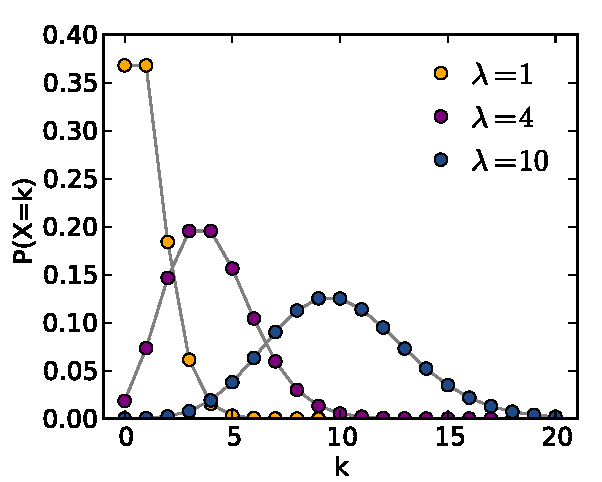
\includegraphics[width = 3.3cm]{./img/poisson_pmf.pdf}}
	\parbox{3.3cm}{\emph{KVF/CDF:} \\ $F_{\X}[k] =$ zu kompliziert \\ 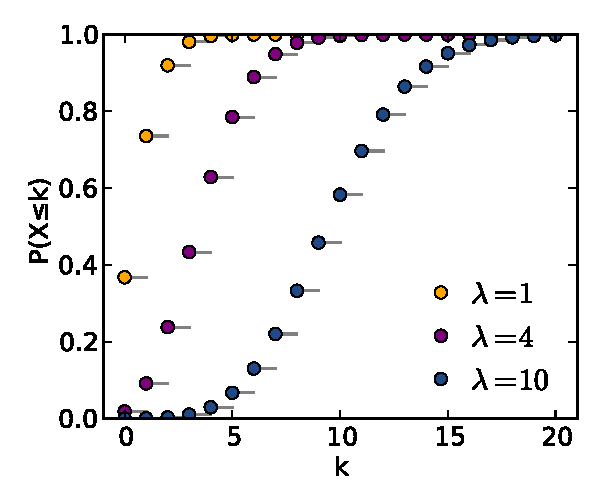
\includegraphics[width = 3.3cm]{./img/poisson_cdf.pdf}}\\
	
	\everymath{\displaystyle}
	\begin{tablebox}{l@{\extracolsep\fill}ll}
		$\underset{\text{Erwartungswert}}{\E[\X] =\lambda}\quad$ & $\underset{\text{Varianz}}{\Var[\X] =\lambda}$ & $\underset{\text{Wahrscheinlichkeitserz. Funktion}}{G_X (\cx s) = e^{\lambda(\cx s-1)}}$\\ 
	\end{tablebox} \everymath{\textstyle}	
	\emph{Charakteristische Funktion}
	\qquad$\varphi_{\X}(\cx s)=\exp\big(\lambda(e^{\cx s} -1)\big)$\\
	\emph{Beispiele:} Zahl der Phänomene in einem Zeitintervall, Google-Anfragen in einer Stunde, Schadensmeldungen an Versicherungen in einem Monat
\end{sectionbox}

% ====================================================================================		
\begin{sectionbox}
	\subsection{Geometrische Verteilung ($p \in [0,1]$)}
	Erster Erfolg eines Bernoulli-Experiments beim $k$-ten Versuch, Gedächtnislos\\[0.5em]
	\parbox{3.3cm}{\emph{WMF/PMF:} \\ $p_{\X}[k] = (1 - p)^{k - 1}p$, $k \in \N$ \\ 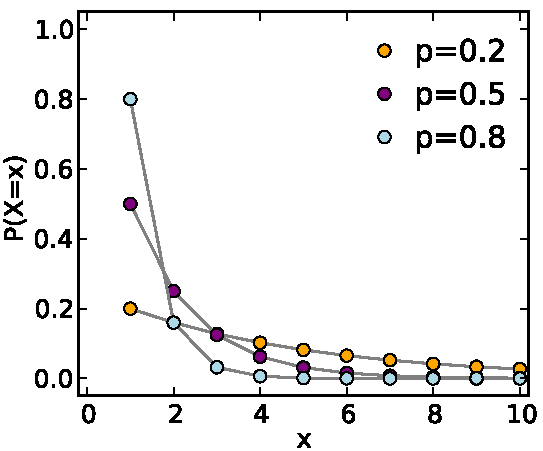
\includegraphics[width = 3.3cm]{./img/geometric_pmf.pdf}}
	\parbox{3.3cm}{\emph{KVF/CDF:} \\ $F_{\X}[k] = 1-(1 - p)^k$, $k \in \N$ \\ 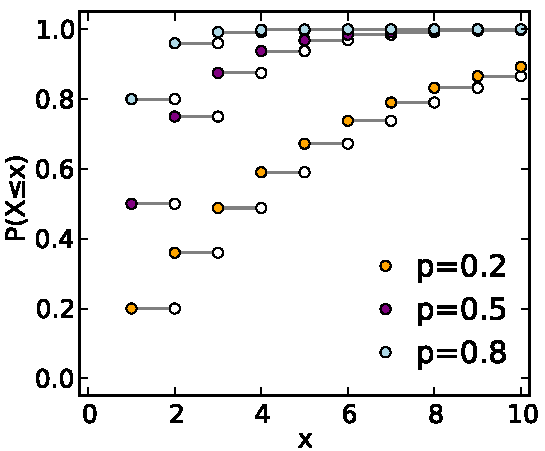
\includegraphics[width = 3.3cm]{./img/geometric_cdf.pdf}}\\
	
	
	\everymath{\displaystyle}
	\begin{tablebox}{l@{\extracolsep\fill}ll}
		$\underset{\text{Erwartungswert}}{\E[\X] =\frac{1}{p}}$ & $\underset{\text{Varianz}}{\Var[\X] =\frac{1-p}{p^2}}$ & $\underset{\text{Wahrscheinlichkeitserz. Funktion}}{G_X (z) = \frac{pz}{1-z+pz}}$\\ 
	\end{tablebox} 
	\emph{Charakteristische Funktion}
	\qquad $\varphi_{\X}(\cx s) = \frac{p e^{\i \cx s}}{1-(1-p)e^{\i \cx s}}$\\
	\emph{Beispiele:} diskrete Dauer bis ein technisches Gerät zum ersten Mal ausfällt, Anzahl der Würfe bis man eine "6" würfelt
\end{sectionbox}

% ====================================================================================
\begin{sectionbox}
	\subsection{Exponentialverteilung ($\lambda > 0$)}
	Wie geometrische Verteilung für stetige Zufallsvariablen ("'Lebensdauer"'), Gedächtnislos\\[0.5em]
	\parbox{3.3cm}{\emph{WDF/PDF:}\\ $f_{\X}(x) = \lambda e^{-\lambda x}$ \qquad$x \geq 0$\\ 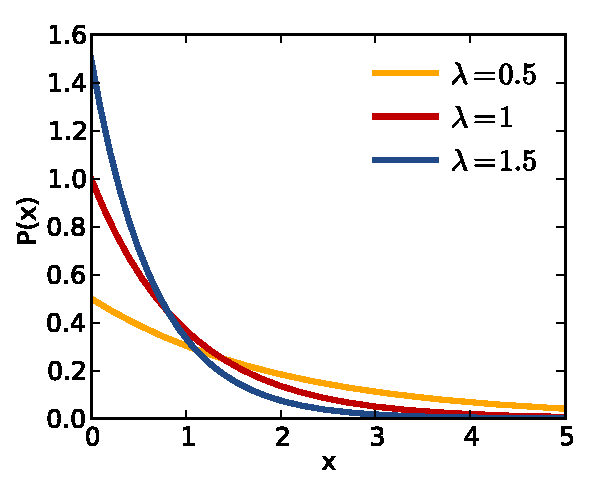
\includegraphics[width = 3.3cm]{./img/exponential_pdf.pdf}}
	\parbox{3.3cm}{\emph{KVF/CDF:} \\ $F_{\X}(x) = 1-e^{-\lambda x}$ \qquad$x \geq 0$ \\ 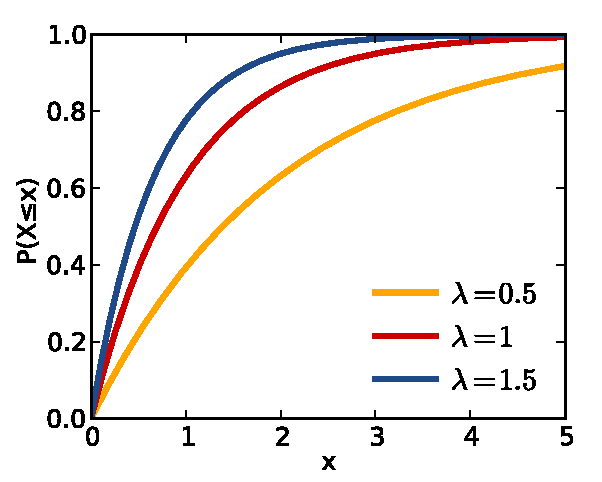
\includegraphics[width = 3.3cm]{./img/exponential_cdf.pdf}}\\
	\everymath{\displaystyle}
	\begin{tablebox}{l@{\extracolsep\fill}ll}
		$\underset{\text{Erwartungswert}}{\E(\X) =\frac{1}{\lambda}}$ & $\underset{\text{Varianz}}{\Var(\X) =\frac{1}{\lambda^2}}$ & $\underset{\text{Charakt. Funktion}}{\varphi_{\X}(\omega) = \frac{\lambda}{\lambda-j\omega}}$\\ 
	\end{tablebox}
	\emph{Beispiele:} Lebensdauer von el. Bauteilen, Zeitdauer zwischen zwei Anrufen in einem Call-Center
\end{sectionbox}

\begin{sectionbox}
	\subsection{Normalverteilung ($\mu \in \R , \sigma > 0$)}
	\parbox{3.3cm}{\emph{WDF/PDF:} \\ 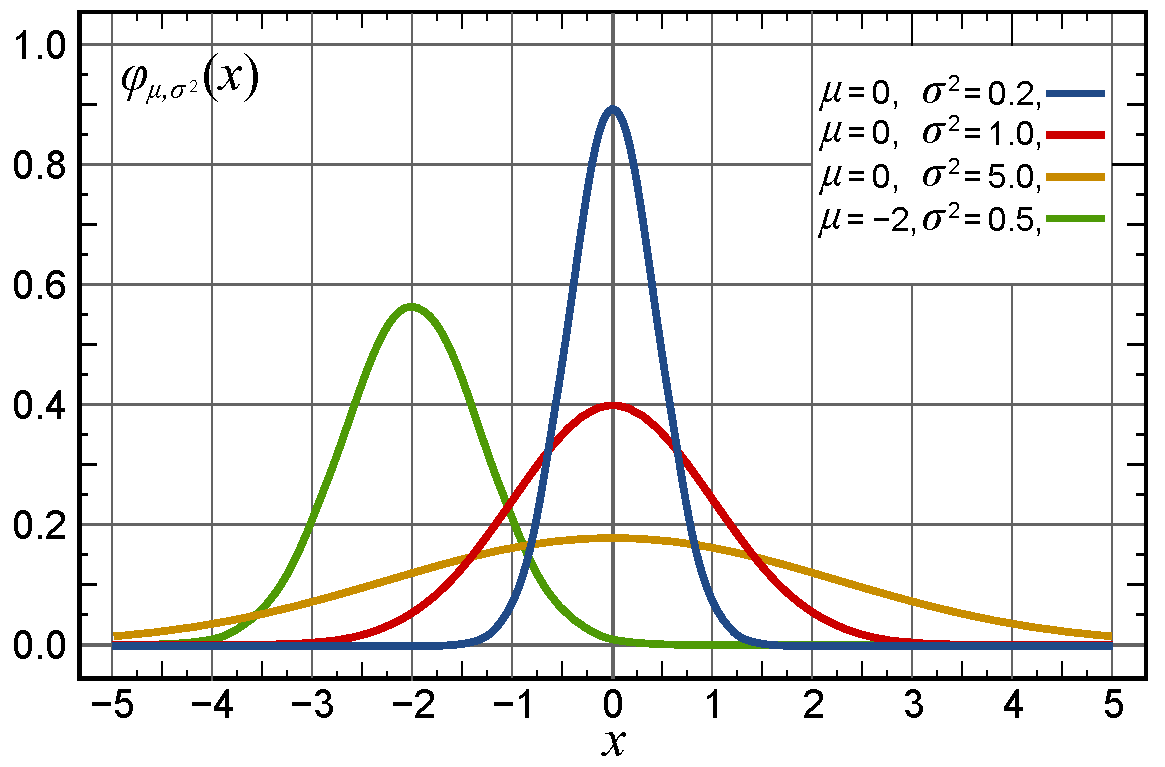
\includegraphics[width = 3.3cm]{./img/normal_pdf.pdf}}
	\parbox{3.3cm}{\emph{KVF/CDF:} \\ 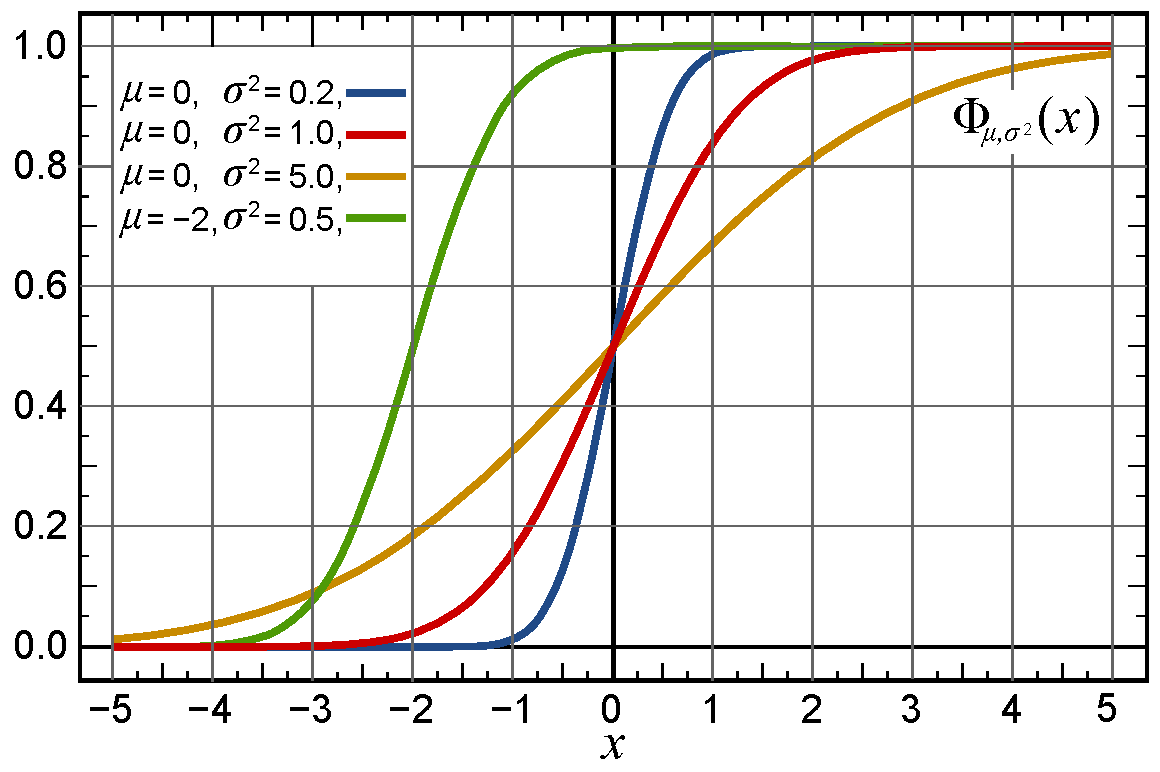
\includegraphics[width = 3.3cm]{./img/normal_cdf.pdf}}\\
	\paragraph{WDF}
	\boxed{f_X (x) = \frac{1}{\sqrt{2 \pi \sigma^2}} e^{-\frac{(x-\mu)^2}{2 \sigma^2}} \quad x \in \mathbb R}
	
	\everymath{\displaystyle}
	\begin{tablebox}{l@{\extracolsep\fill}ll}
		$\underset{\text{Erwartungswert}}{\E(\X) = \mu}$ & $\underset{\text{Varianz}}{\Var(\X) =\sigma^2}$ & $\underset{\text{Charakt. Funktion}}{\varphi_{\X}(\omega) = e^{j\omega\mu-\frac{\omega^2\sigma^2}{2}}}$\\ 
	\end{tablebox}
	\emph{Schreibweise} $\X \sim \mathcal{N} (\mu,\sigma^2)$ \\
	\emph{Beispiele:} Rauschen, Ort eines Teilchens relativ zu seiner Anfangsposition bei brownscher Molekularbewegung, abgefahrene Sachen, die man nicht genauer bestimmen will oder kann
	\subsubsection{Standartnormalverteilung}
	ist der Spezialfall $\X \sim \mathcal{N} (0,1)$\\
	$\phi(x) = \frac{1}{\sqrt{2\pi}}e^{{-\frac{x^2}{2}}}$\\
	Es gilt außerdem:
	\begin{itemize}
		\item $\Y \sim \mathcal{N}(\mu,\sigma^2) \Ra \X = \frac{1}{\sigma}(\Y - \mu) \sim \mathcal{N}(0,1)$
		\item $\X \sim \mathcal{N}(0,1) \Ra \Y = \sigma \X + \mu \sim \mathcal{N}(\mu,\sigma^2)$
	\end{itemize}
\end{sectionbox}

% ====================================================================================
%\begin{sectionbox}
%	\subsection{Multivariante Normalverteilung}
%	Verbund -WDF: \\
%	$f_{\X_1..\X_n} (x_1..x_n) = \frac{1}{\sqrt{2 \pi}^n \sqrt{\det \ma C}} e^{(- \frac{1}{2} (x - \mu)^\top \ma C^{-1} (x - \mu))}$
%\end{sectionbox}


%\vfill 
\columnbreak
% ----------------------------------------------------------------------------
% | Erwartungswert und Varianz |
% ~~~~~~~~~~~~~~~~~~~~~~~~~~~~~~~~~~~~~~~~~~~~~~~~~~~~~~~~~~~~~~~~~~~~~~~~~
% SECTION ====================================================================================
\section{Erwartungswert}
% ============================================================================================
\begin{sectionbox}
	\subsection{Erwartungswert}
	gibt den mittleren Wert einer Zufallsvariablen an

	\begin{emphbox}
		$\E [\X] = \underset{\text{diskrete} \X:\Omega \ra \Omega'}{\sum\limits_{x \in \Omega'} x \cdot \P_{\X}(x)} \quad \stackrel{\wedge}{=}\quad \underset{\text{stetige} \X: \Omega \ra \R}{\int \limits_{\R} x \cdot f_{\X} (x) \diff x}$
	\end{emphbox}
	Eigenschaften:
	\begin{tablebox}{ll}	
		Linearität: &
		$E[\alpha \X + \beta \Y] = \alpha E [\X] + \beta E[\Y]$ \\ 
		Monotonie: & 
		$\X \le \Y \Ra E[\X] \le E[\Y]$ \\
	\end{tablebox}
	Beweis mit der Definition und der Linearität des Integrals bzw. der Summe. \\ 
	\\
	$\E[\X\Y] = \E[\X] \E[\Y]$, falls $\X$ und $\Y$ stochastisch unabhängig\\
	Umkehrung nicht möglichich: Unkorrelliertheit $\not \Ra$ Stoch. Unabhängig! \\
	\\
	Spezialfall für $\X: \Omega \ra \mathbb R_+$: \\
	$\E[\X] = \int \limits_0^\infty \P(\X > t) \diff t$ (stetig) \qquad $\E[\X] = \sum \limits_{k=0}^{\infty} \P(\X >k)$ (diskret)

	\subsubsection{Für Funktionen von Zufallsvariablen $g: \mathbb R \ra \mathbb R$}
	$\E[g(\X)] = \sum \limits_{x \in \Omega'} g(x) \P_{\X} (x)\quad \stackrel{\wedge}{=}\quad \int \limits_{\R} g(x) f_X (x) \diff x$
\end{sectionbox}

% \begin{sectionbox}
% 	\subsection{diskrete (reelle) Zufallsvariablen}
% 	\boxed{\E [\X] = \sum \limits_{x \in \Omega'} x \P(\{ \X = x \}) = \sum \limits_{x \in \Omega'} x p_x (x)} \\
% 	für $\X: \Omega \ra \Omega' \subset \mathbb R$ 
	
% 	Für Funktionen von Zufallsvariablen:
	
% 	$\E[\Y] = E[g(\X)] = \sum \limits_{x \in \Omega'} g(x) p_{\X} (x)$\\
% 	mit $\X : \Omega \ra \Omega' \subset \mathbb R$ und $g: \mathbb R \ra \mathbb R$
% \end{sectionbox}

% \begin{sectionbox}
% 	\subsection{stetige Zufallsvariablen}
% 	\boxed{\E[\X] = \int \limits_\mathbb R x \cdot f_{\X} (x) \diff x} für $\X : \Omega \ra \mathbb R$
	
% 	Für Funktionen von Zufallsvariablen:
	
% 	$\E[\Y] = E[g(\X)] = \int \limits_{\mathbb R} g(x) f_X (x) \diff x$\\
% 	mit $\X : \Omega \ra \mathbb R $ und $g: \mathbb R \ra \mathbb R$
% \end{sectionbox}

% \begin{sectionbox}
% 	\subsection{Eigenschaften des Erwartungswerts}
	
% 	\begin{tablebox}{ll}	
% 		Linearität: &
% 		$E[\alpha \X + \beta \Y] = \alpha E [\X] + \beta E[\Y]$ \\ 
% 		Monotonie: & 
% 		$\X \le \Y \Ra E[\X] \le E[\Y]$ \\
% 	\end{tablebox}
% 	Beweis mit der Definition und der Linearität des Integrals bzw. der Summe. \\ 
	
% 	Falls $\X$ und $\Y$ stochastisch unabhängig:
% 	$\E[\X\Y] = \E[\X] \E[\Y]$ \\
% 	Achtung: Umkehrung nicht möglich. \\ 
% 	Stoch. Unabhängig $\Ra$ Unkorrelliertheit \\
% 	\\
	
% 	Spezialfall für $\X: \Omega \ra \mathbb R_+$: \\
% 	$\E[\X] = \int \limits_0^\infty \P(\X > t) \diff t$ (stetig) \qquad $\E[\X] = \sum \limits_{k=0}^{\infty} \P(\X >k)$ (diskret)
% \end{sectionbox}

\vfill
%\columnbreak

% SECTION ====================================================================================
\section{Varianz und Kovarianz}
% ============================================================================================
\begin{sectionbox}
\subsection{Varianz}
	ist ein Maß für die Stärke der Abweichung vom Erwartungswert
	\begin{emphbox}
		$\Var [X] = \E \big[(\X - \E[\X])^2\big] = \E[\X^2] - \E[\X]^2$ 
	\end{emphbox}
	$\Var [ \alpha \X + \beta] = \alpha^2 \Var [\X]$ \hfill $\Var [\X] = \Cov [\X,\X]$\\[0.5em]
	$\Var \left[\sum \limits_{i=1}^n \X_i \right] = \sum \limits_{i=1}^{n} \Var [\X_i] + \sum\limits_{j \not= i} \Cov[\X_i, \X_j]$
	\subsubsection{Standard Abweichung}
	$\sigma = \sqrt{\Var[\X]}$	
\end{sectionbox}

\begin{sectionbox}
\subsection{Kovarianz}
	Maß für den linearen Zusammenhang zweier Variablen
	\begin{emphbox}
		$\Cov [\X,\Y] = \E[(\X- \E[\X])(\Y - \E[\Y])] = \Cov [\Y, \X]$\\[0.5em]
		$\Cov [\X,\Y] = \E [\X\Y] - \E[\X] \E[\Y] = \Cov[\Y, \X]$
	\end{emphbox}
	$\Cov [\alpha \X + \beta, \gamma \Y + \delta] = \alpha \gamma \Cov [\X, \Y]$ \\
	$\Cov [ \X + \textit U, \Y + \textit V] = \Cov [\X, \Y] + \Cov [\X, \textit V] + \Cov [\textit U, \Y] + \Cov [\textit U, \textit V]$ \\

	\subsubsection{Korrelation = standardisierte Kovarianz}
	$\rho(\X,\Y) = \frac{\Cov[\X,\Y]}{\sqrt{\Var[\X] \cdot \Var[\Y]}} = \frac{C_{x,y}}{σ_x \cdot σ_y}$ \qquad $\rho(\X,\Y) ∈ [-1;1]$
\end{sectionbox}


\begin{sectionbox}
	\subsection{Unkorreliertheit}
	wenn gilt:
	\begin{emphbox}
		$\Cov [\X,\Y] = 0 \Leftrightarrow \E[\X\Y] = \E[\X] \E[\Y]$
	\end{emphbox}
	Stoch. Unabhängig $\Ra$ Unkorrelliertheit \\\\
	wenn ZV normalverteilt (sonst nicht!):\\
	Unkorreliertheit $\Ra$ stoch. Unabhängigkeit\\\\
	bei paarweisen unkorrellierten Zufallsvariablen:\\
	$\Var[\sum \limits_{i=1}^{n} \X_i] = \sum \limits_{i=1}^{n} \Var [\X_i]$
\end{sectionbox}

\begin{sectionbox}
	\subsection{Orthogonalität}
	
	\begin{emphbox}
		$\E[\X\Y] = 0$
	\end{emphbox}
	mit dem Korrelationswert $\E[\X\Y]$
	
\end{sectionbox}

\begin{sectionbox}
	\subsection{Korrelationskoeffizient}
	$\rho_{\X,\Y} = \frac{\Cov[\X,\Y]}{\sqrt{\Var[\X]} \sqrt{\Var[\Y]}} = \frac{c_{\X,\Y}}{\sigma_{\X} \sigma_{\Y}}$ mit $\rho_{\X, \Y} \in [-1,1]$\\ \\
	Korrelationskoeffizient von $\mathsf X$ und $\mathsf Y$\\\\
	Es gilt: $\begin{cases}\text{negativ korreliert} & \rho_{\mathsf{\X,\Y}}\in [-1,0) \\ 
	\text{unkorreliert} & \rho_{\mathsf{\X,\Y}}=0 \\ 
	\text{positiv korreliert} & \rho_{\mathsf{\X,\Y}}\in (0,1]\end{cases}$
\end{sectionbox}

%TODO: Lineare Regression hier einfügen


%\begin{sectionbox}
%	\subsection{Komplexe Zufallsvariablen}
%	$\cx{\Z} = \X + \i \Y$ \qquad $\cx{\W} = \U + \i \Y$\\
%	$\E[\Z] = \E[\X + \i \Y] = \E[\X] + \i \E[\Y]$\\
%	$\Var[\Z] = \E [(\Z - \E[\Z])^2] = \E[\Z^2] - \E[\Z]^2$\\
%	$\Cov[Z,W] = \E[\Z\W^*] - \E[\Z]\E[\W]^* = \Cov[W,Z]^*$
%\end{sectionbox}



\vfill %\textcolor{red}{Bild von der Standardabweichung}

% SECTION ====================================================================================
\section{Erzeugende und charakter. Funktionen}
% ============================================================================================

\begin{sectionbox}
	\subsection{Wahrscheinlichkeitserzeugende Funktion} 
	für $\X : \Omega \ra \mathbb N_0$
	
	\boxed{G_{\X} (z) = \E[z^{\X}] = \sum \limits_{k=0}^\infty p_{\X} (k) z^k, \quad \abs{z} \le 1}
	
	\paragraph{Anwendungen}
	\begin{eqnarray*}
		p_{\X}(n) =\P(\eset{\X = n}) = \frac{1}{n!} [\frac{\diff^n}{\diff z^n} G_{\X} (z)]_{z = 0}, \quad \forall n \in \mathbb N_0 \\
		\E [\X] = [\frac{\diff}{\diff z} G_{\X} (z)]_{z = 1} \\
		\E [\X^2]-\E[\X] = [\frac{\diff^2}{\diff z^2} G_{\X} (z)]_{z = 1} \\
		\Var [\X] =[\frac{\diff^2}{\diff z^2} G_{\X} (z)]_{z = 1} - \E [\X]^2 + \E [\X] 
	\end{eqnarray*}
	Für $\X_i : \Omega \ra \mathbb N_0, i \in \eset{1, \ldots, n}$ stochastisch unabhängige, diskrete, nichtnegative ZV und $\Z = \sum_{i=1}^{n} \X_i$
	\[G_{\Z} (z) = \prod_{i = 1}^{n} G_{\X_i} (z)\]
	
\end{sectionbox}

% Im WS2015/16 nicht Klausurrelevant
%\begin{sectionbox}
%	\subsection{Momenterzeugende Funktion} % (fold)
%	\label{sub:momenterzeugende_funktion}
%	
%	Mit $\X: \Omega \ra \mathbb R$ eine reelle ZV: \\
%	
%	\boxed{
%		M_{\X} (s) = \E [e^{s \X}], \quad s \in \mathbb D = \eset{s \in \mathbb R }{\E [e^{s \X} < \infty]}
%	}\\ 
%	
%	
%	Potenzreihenentwicklung (mit $s \in ]-a, a[$):\\
%	$M_{\X} (s) = \E [ e^{s \X}] = \E \left[\sum \limits_{k=0}^{\infty} \frac{s^k}{k!} \X^k\right] = \sum \limits_{k=0}^{\infty} \frac{s^k}{k!} \E\left[\X^k\right]$
%	
%	Erwartungswert:
%	$\E[\X^n] = \left[\frac{\diff^n}{\diff s^n} M_{\X} (s)\right]_{s=0}, \quad \forall n \in \mathbb N_0$
%	
%	Summe von ZV:
%	$M_{\Z} (s) = \prod \limits_{i = 1}^{n} M_{\X_i} (s)$
%\end{sectionbox}

% subsection momenterzeugende_funktion (end)
\begin{sectionbox}
	\subsection{Charakteristische Funktion} % (fold)
	\label{sub:charakteristische_funktion}
	\boxed{\varphi_{\X} (\omega) = \ew{e^{\i \omega \X}} , \quad \omega \in \mathbb R} $\qquad \varphi_{\X} = \int\limits_{-\infty}^\infty e^{\i\omega x} f_{\X}(x) \diff x$\\
	$f_{\X}(-x) \T \varphi(\omega)$ \\
	
	\emph{Erwartungswert:}
	\begin{eqnarray*}
		\E[\X^n] = \frac{1}{\i^n} \left[\frac{\diff^n}{\diff \omega^n} \varphi_{\X}(\omega)\right]_{\omega = 0}
	\end{eqnarray*}
	\emph{Summe von ZV:} $Z=\sum_{i=1}^{n}X_i$
	\begin{eqnarray*}
		\varphi_{\Z} (\omega) = \prod_{i=1}^{n} \varphi_{\X_i} (\omega)
	\end{eqnarray*}
\end{sectionbox}	

% subsection charakteristische_funktion (end)
\begin{sectionbox}
	\subsection{Der zentrale Grenzwertsatz}
	\emph{Definition}: Seien $\X_i, i \in {1,...,n}$, stochastisch unabhängige und identisch
	verteilte reelle Zufallsvariablen und gelte $E[\X_i] = \mu < \infty$ und $Var[\X_i] = \sigma^2 < \infty$. 
	Dann konvergiert die Verteilung der standardisierten Summe\\ 
	\centerline{$\Z_n= \sum\limits_{i=1}^{n}\frac{(\X-\mu)}{\sigma\sqrt{n}}$} \\
	d.h $E[\Z_n] = 0$ und $Var[\Z_n] = 1$, für $n \ra \infty$ gegen die Standartnormalverteilung. \\
	Es gilt also: \\
	\centerline{$\lim_{n \ra \infty} \P({\Z_n \le z}) = \Phi (z)$}
\end{sectionbox}	
% subsection der_zentrale_grenzwertsatz (end)


\vfill
%\columnbreak 

% SECTION ====================================================================================
\section{Reelle Zufallsfolgen}
% ============================================================================================
\begin{sectionbox}
	Eine reelle Zufallsfolge ist ganz einfach eine Folge reeller Zufallsvariablen. \\ \\
	\textbf{Ensemble} \\
	$\textsf{S}_n : \Omega_n \times \Omega_{n-1} \times \dots \times \Omega_1 \ra \R$\\
	$(\omega_n,\omega_{n-1},\dots,\omega_1) \mapsto s_n(\omega_n,\omega_{n-1},\dots,\omega_1), \quad n \in \N$\\
	\emph{Erklärung:} Jede Realisierung von $\textsf{S}_n$ wird erzeugt durch die Menge (das Ensemble) aufeinanderfolgender Realisierungen $\X_k$ mit $k \in \{1,\dots,n\}$. \\ \\	
	\textbf{Pfad} \\
	$\vec{\textsf{S}}_n = (\textsf{S}_n,\textsf{S}_{n-1},\dots,\textsf{S}_1) : \Omega^{(n)} \ra \R^n$\\
	$\vec{\omega}_n \mapsto \vec{s}_n(\vec{\omega}_n) = (s_n(\vec{\omega}_n),s_{n-1}(\vec{\omega}_n),\dots,s_1(\vec{\omega}_n)), \quad n \in \N$\\
	\emph{Erklärung:} Die Abfolge der Realisierungen von $\textsf{S}_1$ bis $\textsf{S}_n$ (also der Pfad von $\textsf{S}$) und somit auch jedes einzelne $\textsf{S}_k$ kann als Ergebnis des Ereignisses $\vec{\omega}_n$ angesehen werden.
\end{sectionbox}

\begin{sectionbox}
	\subsection{Verteilungen und Momente}
	\begin{tablebox}{@{\extracolsep\fill}ll@{}}
		Erwartungswert & $\mu_{\X}(n) = E[\X_n]$\\
		Varianzfolge & $\sigma^2_{\X}(n) = Var[\X_n] = E[\X_n^2] - E[\X_n]^2$\\
		Autokorrelation & $r_{\X}(k,l) = E[\X_k \X_l]$\\
		Autokovarianz & \!\!\!\!\! $c_{\X}(k,l) = Cov[\X_k,\X_l]$ \newline $= r_{\X}(k,l) - \mu_{\X}(k) \mu_{\X}(l)$\\
	\end{tablebox}
\end{sectionbox}

\begin{sectionbox}
	\subsection{Random Walk}
	$n \in \N$ Schritte mit 2 möglichen Bewegungsrichtungen $\X \in \{+\delta,-\delta\}$\\
	\parbox{2cm}{
		\boxed{
			\textsf{S}_n = \sum\limits_{i=1}^{n}{\X_i}
		} } \parbox{4cm}{ $\P\left(\{\X_i = +\delta\}\right) = p$ \\ $\P\left(\{\X_i = -\delta\}\right) = 1 - p$\\ symmetrisch $\Leftrightarrow p = \frac{1}{2}, \ \mu_{\textsf{S}}(n) = 0$\\ }
		
		\begin{tablebox}{@{\extracolsep\fill}ll@{}}
			$E[S] = \mu_{\textsf{S}}(n) = n(2p - 1)\delta$ & $E[\X_i] = (2p - 1)\delta$ \\
			$Var[S] = \sigma^2_{\textsf{S}}(n) = 4np(1 - p)\delta^2$ & $Var[\X_i] = 4p(1 - p)\delta^2$ \\
		\end{tablebox}
	\end{sectionbox}

\begin{sectionbox}
	\subsection{Stationarität}
	Eine Zufallsfolge ist \emph{stationär}, wenn um ein beliebiges $k$ $(k \in \N)$ zueinander verschobene Zufallsvektoren die selbe Verteilung besitzen.\\
	Im \emph{weiteren Sinne stationär (W.S.S.)}, wenn:
	\begin{tablebox}{@{\extracolsep\fill}lll@{}}
		$\mu_{\X}(i) = \mu_{\X}(i + k)$ \\
		$r_{\X}(i_1,i_2) = r_{\X}(i_1 + k,i_2 + k) = r_{\X}(i_1 - i_2)$\\
	\end{tablebox}
	stationär $\Ra$ WSS (aber nicht anders herum!)
\end{sectionbox}

\begin{sectionbox}
	\subsection{Markow-Ungleichung}
	\boxed{\P(\eset{\abs{\X} \ge a}) \le \frac{\E[|\X|]}{a} }
\end{sectionbox}

\begin{sectionbox}
	\subsection{Tschebyschow-Ungleichung}
	\boxed{\P(\eset{\abs{\X- \E[\X]} \ge a}) \le \frac{\Var[\X]}{a^2} }
	
	
\end{sectionbox}
\begin{sectionbox}
	\subsection{Das schwache Gesetz der großen Zahlen}
	Sei $(\X_i : i \in \N)$ eine Folge reeller, paarweise unkorrelierter Zufallsvariablen mit beschränkter Varianz:\\
	$\frac{1}{n} \sum\limits_{i = 1}^n (\X_i - \E[\X_i]) \ra 0$\\ \\
	Für stochastisch unabhängige und identisch verteilte Folgenelemente mit $E[\X_i] = E[X]$ und $Var[\X_i] = Var[X] < \infty$ gilt: \\
	$\frac{1}{n} \sum\limits_{i = 1}^n (\X_i) \ra \E[\X_i] $
\end{sectionbox}

% SECTION ====================================================================================
\section{Markowketten \\ (bedingte Unabhängigkeit: Abschnitt \ref{bed-unabh})}
\begin{sectionbox}
	\subsection{Markowketten}
	\subsubsection{Allgemein}
	Eine Zufallsfolge ($\mathsf{\X}_{n}: n \in \mathbb{N}$) heißt Markowkette, falls $\forall \ n_{i} \in \N, \\
	i \in {1, \dots k}$ mit $n_{1} < \dots < n_{k}$ gilt:\\
	$\mathsf{(\X_{n_{1}},\X_{n_{2}}, \dots \X_{n_{k-2}}) \ra \X_{n_{k-1}} \ra \X_{n_{k}}}$ \\
	$\Ra$ Die Verteilung eines Folgeelements hängt nur vom direkten Vorgänger ab
	\begin{tablebox}{@{\extracolsep\fill}l@{}}
	$p_{\X_{n_k}|\X_{n_{k-1}},\X_{n_{k-2}},...,\X_{n_1}}(x_{n_k}|x_{n_{k-1}},x_{n_{k-2}},...,x_{n_1})$ \\
	$=p_{\X_{n_k}|\X_{n_{k-1}}}(x_{n_k}|x_{n_{k-1}})$ \\
	\end{tablebox}

	\begin{tablebox}{@{\extracolsep\fill}l@{}}
	$f_{\X_{n_k}|\X_{n_{k-1}},\X_{n_{k-2}},...,\X_{n_1}}(x_{n_k}|x_{n_{k-1}},x_{n_{k-2}},...,x_{n_1})$ \\
	$=f_{\X_{n_k}|\X_{n_{k-1}}}(x_{n_k}|x_{n_{k-1}})$
	\end{tablebox}

	\subsubsection{Zustandsübergang}
	\emph{Zustandsübergangswahrscheinlichkeit:} \\ 
	\centerline{$p_{\X_{n} | \X_{n-1}}(x_{n} | x_{n-1})$}\\
	
	\qquad Verbund-WMF: \\
	$p_{\X_1,...,\X_n}(x_1,...,x_n)=p_{\X_1}(x_1)\prod\limits_{i=2}^{n}p_{\X_i|\X_{i-1}}(x_i|x_{i-1})$ \\ 
	
	\emph{Zustandsübergangsdicht:} \\
	\centerline{$ f_{\X_{n} | \X_{n-1}}(x_{n} | x_{n-1})$}\\
	
	\qquad Verbund-WDF: \\
	$f_{\X_1,...,\X_n}(x_1,...,x_n)=f_{\X_1}(x_1)\prod\limits_{i=2}^{n}f_{\X_i|\X_{i-1}}(x_i|x_{i-1})$ \\ \\

	
	Eine Markowkette heißt \emph{homogen}, wenn die Übergangswahrscheinlichkeit\ unabhängig vom Index ist \\
	$p_{\X_{n+1} | \X_{n}} (x_{n+1} | x_{n}) = p_{\X_{n+1+k} | \X_{n+k}} (x_{n+1} | x_{n})$ \\
	$f_{\X_{n+1} | \X_{n}} (x_{n+1} | x_{n}) = f_{\X_{n+1+k} | \X_{n+k}} (x_{n+1} | x_{n})$ \\
	

	\subsubsection{Chapman-Kologorow Gleichung}
	2-Schritt-Übergangswahrscheinlichkeit: \\
	 $p_{\X_{n+2}|\X_n}(x_{n+2}|x_n)= \\ \sum\limits_{\xi\in\mathbb{X}}p_{\X_{n+2}|\X_{n+1}}(x_{n+2}|\xi)p_{\X_{n+1}|\X_n}(\xi |x_n)$
	 
	m+l-Schritt-Übergangswahrscheinlichkeit: \\
	$p_{\X_{n+m+l}|\X_n}(x_{n+m+l}|x_n) =$\\
	\resizebox{\textwidth}{!}{$ \sum\limits_{\xi \in \mathbb{X}}p_{\X_{n+m+l}|\X_{n+m}}(x_{n+m+l}|x_{n+m})p_{\X_{n+m}|\X_{n}}(x_{n+m}|x_{n})$}
\end{sectionbox}
\begin{sectionbox}
	\subsubsection{Markowketten im endlichen Zustandsraum}
	$\vec{p}_{n} \triangleq \begin{bmatrix} p_{\X_{n}}(x_{1}) \\ p_{\X_{n}}(x_{2}) \\ \vdots \\ p_{\X_{n}}(x_{N}) \end{bmatrix} \quad \in [0,1]^{N}\text{ mit }[\vec{p}_{n}]_{i} = p_{\X_{n}}(x_{i})$ \\
	\emph{Übergangsmatrix:}
	 $\Pi = \begin{bmatrix} p_{11} & \cdots & p_{1N} \\ \vdots & \ddots &   \\ p_{N1} & & p_{NN} \end{bmatrix} \quad \in [0,1]^{N \times N}$\\

	 \emph{Übergangswahrscheinlichkeit:} $p_{ij} = p_{\X_{n+1}|\X_n}(\xi_i,\xi_j)$ \\
	 \centerline{Spaltensumme muss immer 1 ergeben!}\\
	 \begin{tablebox}{l}
		 $\vec{p}_{n+1}  = \Pi \vec{p}_{n} \quad n \in \N$ \\
		 $\vec{p}_{n+m}  = \Pi^{m} \vec{p}_{n} \quad n, m \in \N$
	 \end{tablebox}
	 Eine Verteilung heißt \emph{stationär}, wenn gilt:\\
	\[\vec{p}_{\infty}  = \Pi \vec{p}_{\infty} \]
\end{sectionbox}


% SECTION ====================================================================================
\section{Reelle Zufallsprozesse}
% ============================================================================================
\begin{sectionbox}
	\subsection{Ensemble und Musterfunktion}
	\begin{itemize}
		\item Ein Zufallsprozess kann als \emph{Ensemble} einer nicht abzählbaren Menge von Zufallsvariablen $X_{t}$ mit $t \in \mathbb{R}$ interpretiert werden.
		\item Ein Zufallsprozess kann als \emph{Schar von Musterfunktionen} \\ $\X_{t}(\omega) : \mathbb{R} \mapsto \mathbb{R},$
		 mit $\X(\omega)$ als deterministische Funktion von $t$, mit einem gegebenen Ereignis $\omega \in \Omega$ interpretiert werden.
	\end{itemize}
\end{sectionbox}
\begin{sectionbox}
	\subsection{Verteilungen und Momente}
	Zeitlich, Kontinuierlich veränderliche Zufallsvariable $\X_t$\\
	
	\begin{emphbox}
		\raggedright
		\textbf{Erwartungswertfunktion:} \\ $\mu_X (t) = \E[\X_t]$ \\[0.5em]
		\textbf{Autokorrelationsfunktion:} \\ $r_{\X}(s,t) = \E[\X_s \X_t]$\\[0.5em]
		\textbf{Autokovarianzfunktion:} \\ $c_{\X}(s,t) = \Cov(\X_s,\X_t) = r_{\X}(s,t) - \mu_{\X}(s)\mu_{\X}(t)$
	\end{emphbox}	
	\emph{Hinweis:} Bei Integration über $r_{\X}$ immer darauf achten, dass $s - t > 0$. Bei Bedarf Integral aufteilen und Grenzen anpassen.
\end{sectionbox}
\begin{sectionbox}
	\subsection{Stationarität}
	Ein Zufallsprozess ist \emph{stationär}, wenn um ein beliebiges $s$ $(s \in \R)$ zueinander verschobene Zufallsvektoren die selbe Verteilung besitzen.
	\begin{tablebox}{@{\extracolsep\fill}lll@{}}
		$F_{\mathsf{X}_{t_{1}},\dots,\mathsf{X}_{t_{n}}} (x_{1}, \dots x_{n}) = F_{\mathsf{X}_{t_{1}+s},\dots,\mathsf{X}_{t_{n}+s}} (x_{1}, \dots x_{n})$
	\end{tablebox}
	Im \emph{weiteren Sinne stationär (W.S.S.)}, wenn:
	\begin{tablebox}{@{\extracolsep\fill}lll@{}}
		$\mu_{\X}(t) = \mu_{\X}(t + s)$ & $\land$ & $r_{\X}(t_1,t_2) = r_{\X}(t_1 + s,t_2 + s)$\\
	\end{tablebox}
	\textbf{Daraus folgt} mit $s = t + \tau$\\
	$r_{\X}(s,t) = \E[\X_s \X_t] = \E[\X_{t+\tau} \X_t] = r_{\X}(s -t) = r_{\X}(\tau)$
	
	
	Im \emph{weiteren Sinne zyklisch stationär}, wenn:
	\begin{tablebox}{@{\extracolsep\fill}lll@{}}
		$\mu_{\X}(t) = \mu_{\X}(t + T)$ & $\land$ & $r_{\X}(t_1,t_2) = r_{\X}(t_1 + T,t_2 + T)$\\
	\end{tablebox}
	stationär $\Ra$ WSS $\Ra$ im weiteren Sinne zyklisch stationär (aber nicht anders herum!)
\end{sectionbox}
\begin{sectionbox}
	\subsection{Mehrere Zufallsvariablen auf dem selben Wahrscheinlichkeitsraum}
	\begin{emphbox}
		\raggedright
		\textbf{Kreuzkorrelationsfunktion:} \\ $r_{\X,\Y}(s,t) = \E[\X_s \Y_t] = r_{\Y,\X}(t,s)$\\
		\textbf{Kreuzkovarianzfunktion:}\\ $c_{\X,\Y}(s,t) = r_{\X,\Y}(s,t) - \mu_{\X}(s)\mu_{\Y}(t) = c_{\Y,\X}(t,s)$
	\end{emphbox}
	
	\subsubsection{Gemeinsame Stationarität}
	Zwei Zufallsprozesse auf demselben Wahrscheinlichkeitsraum sind \emph{gemeinsam stationär}, wenn die einzelnen ZPs jeweils selbst stationär sind und ihre gemeinsamen Verteilungen verschiebungsinvariant sind.
	
	\subsubsection{Gemeinsam im weiteren Sinne stationär}
	\textbf{Voraussetzung:} $\X_t$ und $\Y_t$ sind gemeinsam WSS wenn,\\
	
	\begin{emphbox}
		\raggedright
		$\X_t$ und $\Y_t$ einzelnd WSS und\\
		$r_{\X,\Y}(t_1,t_2) = r_{\X,\Y}(t_1 + s,t_2 + s)$\\
		gemeinsam stationär $\Ra$ gemeinsam WSS (aber nicht umgekehrt!)
	\end{emphbox}
	\textbf{Daraus folgt} mit $s = t + \tau$\\
	$r_{\X}(s,t) = \E[\X_{t+\tau} \X_t] = r_{\X}(\tau) = r_{\X}(-\tau)$ \qquad $r_{\X}(\tau) \le r_{\X}(0)$\\
	$r_{\X,\Y}(\tau)=\E[\X_{t+\tau} \Y_t]=\E[\Y_t \X_{t+\tau}]=r_{\Y,\X}(-\tau)$
	\subsubsection{Stochastische Unkorreliertheit}
	$c_{\X,\Y}(s,t) = 0 \Leftrightarrow r_{\X,\Y}(s,t) = \mu(s)\mu(t), \quad \forall s,t \in \R$
	\subsubsection{Orthogonalität}
	$r_{\X,\Y}(s,t) = 0, \quad \forall s,t \in \R$
\end{sectionbox}

\begin{sectionbox}
	\subsection{Wiener-Prozess ($\sigma > 0$)}
	Als Basis benutzen wir den Random Walk. Durch Multiplikation mit einer Heaviside-Funktion wird der Random Walk zeitkontinuierlich:\\
	\parbox{3cm}{$\textsf{S}_n = \sum\limits_{i=1}^{n}\X_i$ \qquad \qquad $\Ra$}
	\parbox{3.5cm}{$\textsf{S}_t  = \sum \limits_{i=1}^{n}\X_iu(t-iT) \qquad T > 0$}\\ \\
	Für n $\ra \infty$ und T $\ra 0$, mit Schrittweite $\delta = \sqrt{\sigma^2 T}$ folgt der Wiener Prozess: $ \W_t$\\
	\begin{tablebox}{@{\extracolsep\fill}l@{}}
		$f_{\W_t}(w) = \frac{1}{\sqrt{2 \pi \sigma^2 t}} \exp\left( -\frac{w^2}{2 \sigma^2 t} \right)$\\
	\end{tablebox}
\paragraph{Eigenschaften}
\begin{itemize}
	\item Kein Zählprozess!
	\item $ \P(\{\W_0  = 0 \})  = 1$
	\item hat unabhängige Inkremente $\ra r_{xy} (s,t) = 0$
	\item $\W_t \sim \mathcal{N}(0,\sigma^2t), \forall 0 \le t$
	\item $\W_t - \W_s \sim \mathcal{N}(0,\sigma^2(t-s)), \forall 0 \le s \le t$
	\item $\W_t(\omega)$ ist eine stetige Musterfunktion mit Wahrscheinlichkeit 1
\end{itemize}

\begin{tablebox}{@{\extracolsep\fill}ll@{}}
	Erwartungswertfunktion. & $\mu_{\W}(t) = 0$\\
	Varianz & $\sigma_W^2(t) =  \sigma^2 t$ \\
	Autokorrelationsfunktion & $r_{\W}(s,t) = \sigma^2 min\{s,t\}$\\
	Autokovarianzfunktion & $c_{\W}(s,t) = \sigma^2 min\{s,t\}$ \\ 
\end{tablebox}

\end{sectionbox}

%\vfill
%\columnbreak
\begin{sectionbox}
	\subsection{Poisson-Prozess ($N_t: \in \mathbb R_+$)}
	Beim Poisson-Prozess wird der \emph{Zeitpunkt} der Sprünge durch ZV modelliert, nicht die Amplitude. \\
	$ N_t  = \sum \limits_{i=1}^{\infty}u(t-T_i) , \quad T_i = \sum \limits_{j=1}^i \X_j $\\
	$\X_j$ ist exponentiell verteilt, $T_i$ ist Gamma-verteilt
	\begin{tablebox}{@{\extracolsep\fill}l@{}}
		$f_{T_i}(t) = \frac{\lambda^i}{(i-1)!}t^{i-1}e^{-\lambda t}, \quad t \ge 0$\\
		$\P\left(\{N_t = n\}\right) = \frac{(\lambda t)^n}{n!}e^{-(\lambda t)}, \quad \forall n \in \N, t \in \R_+$\\
	\end{tablebox}

\paragraph{Eigenschaften}
\begin{itemize}
	\item ist ein Zählprozess
	\item ist Gedächtnislos
	\item hat unabhängige Inkremente
	\item $N_t - N_s$ ist Poisson-verteilt mit Parameter $(\lambda(t-s)$ für alle $0 \le s \le t$
	\item hat eine Rate $\lambda$
	\item Zeitintervalle zwischen den Inkremetierungen sind unabhängig und identisch exponentialverteilt mit Parameter $\lambda$
	
\end{itemize}


\begin{tablebox}{@{\extracolsep\fill}ll@{}}
	Erwartungswertfunktion & $\mu_N(t) = \lambda t$\\
	Varianz & $\sigma_N^2(t)=\lambda t $\\
	Autokorrelationsfunktion & $r_N(s,t) = \lambda \min\{s,t\} + \lambda^2 st$\\
	Autokovarianzfunktion & $c_N(s,t) = \lambda \min\{s,t\}$ \\ 
\end{tablebox}
\end{sectionbox}

\section{Bedingte Unabhängigkeit}
\label{bed-unabh}
\begin{sectionbox}
	\subsection{Bedingte Unabhängigkeit}
	A und C heißen bedingt unabhängig gegeben B, wenn gilt:\\
	$\P(A \cap C | B) = \P(A | B)\P(C| B)$	bzw.\\
	$\P(A | B \cap C) = \P(A | B)$ \\ \\
	Dann gilt: \\
	$p_{\Z|\Y,\X}(y|y,x) = p_{\Z|\Y}(z|y)$ \\
	$f_{\Z|\Y,\X}(z|y,x) = f_{\Z|\Y}(z|y)$ \\
	$\X,\Z$ sind bedingt unabhängig gegeben $\Y$, kurz: $\X \ra \Y \ra \Z$
\end{sectionbox}

\vfill
% SECTION ====================================================================================
\section{Zufallsprozesse(ZP) und lineare Systeme}
% ============================================================================================
\begin{sectionbox}
	\subsection{Allgemeines}
	Im \emph{Zeitbereich}:\\
	$\text{w}(t)  =  (h \ast v)(t) = \int\limits_{- \infty}^{\infty} h(t - \tau) v(\tau) \, \diff\tau$ \\
	Im \emph{Frequenzbereich:}\\
	$W(f) = H(f)V(f)$ \\ \\
	\parbox{3.8cm}{\boxed{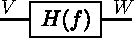
\includegraphics{./img/lds.pdf}}}
	\parbox{3.5cm}{$\textsf{W}_t$  \,\,\,\,\,\,\,\,  Ausgang\\
		$\textsf{V}_t$  \qquad Eingang\\
		$h(s,t)$  Impulsantwort}	\\ \\
	Falls Zufallsprozesse \emph{WSS}: \\
	\emph{Erwartungswert:} $\mu_{\textsf{W}} = \mu_{\textsf{V}} \int\limits_{\infty}^{-\infty} h(t) \diff t$\\
	\emph{Kreuzkorrelationsfkt:} $r_{\textsf{W},\textsf{V}}(\tau) = \E [\textsf{W}_s \textsf{V}_t] =  (h * r_{\textsf{V}})(\tau)$\\
	\emph{Autokorrelationsfkt:} $r_{\textsf{W}}(\tau) = \E [\textsf{W}_s \textsf{W}_t] = (\tilde h * h * r_{\textsf{V}})(\tau)$\\ 
	 mit $\tilde h (\tau) = h(-\tau)$
\end{sectionbox}

\begin{sectionbox}
	\subsection{Leistungsdichtespektrum (LDS)}
	
	\begin{emphbox}
		Nicht WSS $\Ra$ Kein LDS
		
	\end{emphbox}
	
	\parbox{3.8cm}{\boxed{S_{\textsf{V}}(f)  = \int \limits_{-\infty}^{\infty} r_{\textsf{V}}(\tau) e^{-j2\pi f \tau} \diff \tau}}
	\parbox{3.5cm}{$r_{\textsf{V}}(\tau) \T S_{\textsf{V}}(f)$\\
		$r_{\textsf{V},\textsf{W}}(\tau) \T S_{\textsf{V},\textsf{W}}(f)$\\
		$r_{V,W}(-\tau) \T S^*_{V,W}(f)$\vspace{0.3em}}\\
	Auf Frequenz bezogene Signalleistung für infitisimales Frequenzband.\\
	
	\begin{tablebox}{@{\extracolsep\fill}ll@{}}
		$S_{\mathsf{Y}}(f) = |H(f)|^{2} S_{\mathsf{X}}(f)$\\
		$S_{\mathsf{Y,X}}(f) = H(f) S_{\mathsf{X}}(f)$ \\
		$S_{\mathsf{X,Y}}(f) = H^{*}(f) S_{\mathsf{X}}(f)$
	\end{tablebox}
	\parbox{\columnwidth}{ 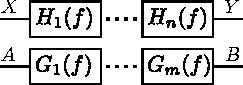
\includegraphics{./img/kreuzlds.pdf}}
	
	$S_{\Y,\X}(f) = (\prod \limits_{i=1}^{n} H_i(f)) S_{\X}(f)$ \quad
	$S_{\X,\Y}(f) = (\prod \limits_{i=1}^{n} H_i^*(f)) S_{\X}(f)$\\
	$S_{\Y,\textsf{B}}(f) = (\prod \limits_{i=1}^{n} H_i(f))(\prod \limits_{j=1}^{m} G_j(f))^* S_{\X,\textsf{A}}(f)$
	
	
	
	\begin{tablebox}{@{\extracolsep\fill}c@{}}
		$S_{\X}(f) = S_{\X}^*(f) \quad \& \quad S_{\X,\Y}(f) = S_{\Y,\X}^*(f), \quad \forall f \in \mathbb R$ \\
		$S_{\X}(f) = S_{\X}(-f), \quad \forall f \in \mathbb R$\\[0.1em]
		$\int \limits_{-\infty}^{\infty} S_{\X}(f) \diff f = r_{\X}(0) = \Var[\X] + \E[\X]^2 = \sigma^2_{\X} + \mu^2_{\X}$\\[0.1em]  %$\left. \int \limits_{-\infty}^{\infty} S_{\X}(f) e^{j2\pi f\tau} \diff f \right|_{\tau = 0} =
		$S_{\X}(f) \ge 0,\quad \forall f \in \mathbb R$ \\
	\end{tablebox}
	
\end{sectionbox}

Momenterzeugende Funktion, Multivariate Normalverteilung, Multivariate reelle Zufallsvariablen und Komplexe Zufallsvariablen waren im WS 2015/16 nicht prüfungsrelevant und werden hier deshalb nicht behandelt.
P.S. Stochastik $\heartsuit$ dich.



% Dokumentende
% ======================================================================
\end{document}
